\problemname{Candy Crush}

In this problem we will play a very simplified version of a popular computer game that we can call Candy Crush. In our version, the playing field is a single stack of $R$ cells. Each cell contains a candy that can be one of three types (let us call them A, B, and C). In the game you may make up to $N$ moves. In each move you swap two adjacent candies so that a sequence of at least three identical candies is formed. If you cannot make any move, the game is over.

After making a move, all candies that are part of such a sequence are crushed (removed). Note that there may be multiple sequences and they all disappear simultaneously. After that, all gaps are filled by candies above falling down (see the figure below). New candies always fill in from above so that the playing field is full. To know which new candies fall in from above, imagine that the original stack is copied upward in an infinitely tall stack (see the figure below).

After the gaps have been filled, a new situation arises and the process repeats automatically: all candies that are part of sequences disappear and the gaps are filled. This continues until no sequences remain on the playing field. Then it is time to make the next move.

The scoring of the game is simple. Every time a sequence of at least three candies is formed (by your move or by falling), you receive $(2L-5)$ points where $L$ is the length of the sequence. A sequence of three candies thus gives 1 point, one with four candies gives 3 points, and so on.

Write a program that, given the original stack and the maximum number of moves you may make, computes the maximum score you can achieve.

\begin{figure}[ht!]
\centering
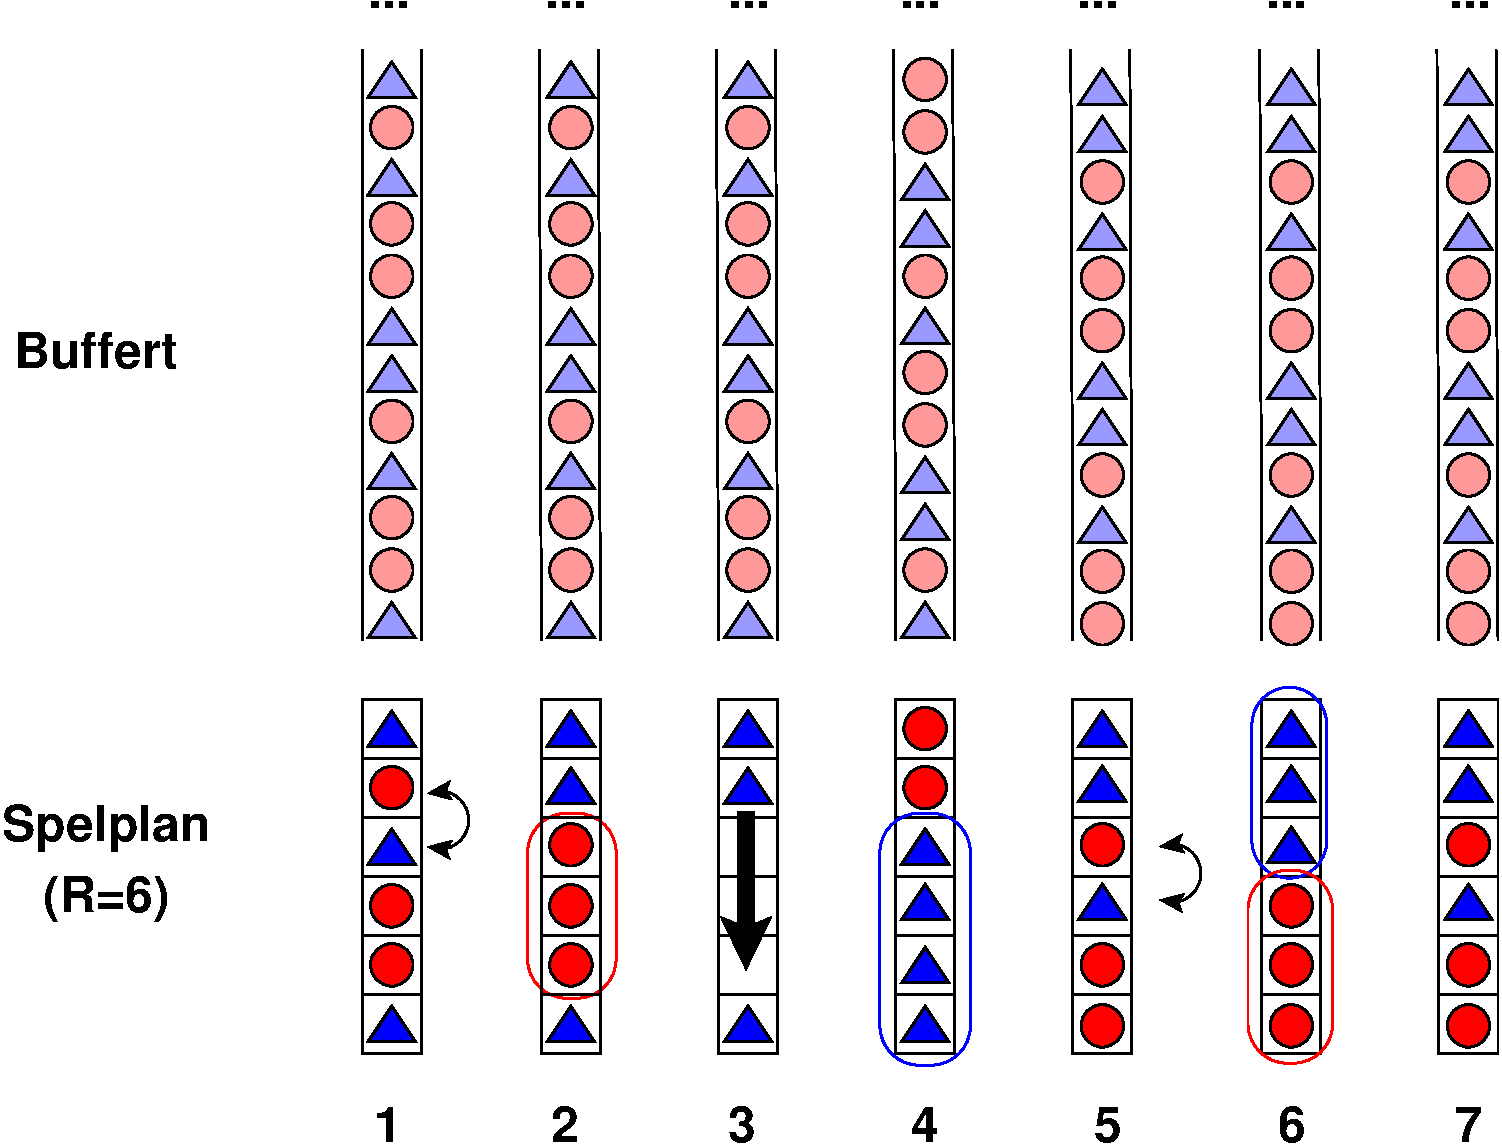
\includegraphics[width=0.7\textwidth]{godiskross_exempel.pdf}
\caption{The sequence of events in the first example (pictures 1--5) and the second example (pictures 1--7). In the input, red circles are called A and blue triangles B. The upper part of the figure symbolizes an imaginary buffer of candies that fall down when candies are crushed. In the initial position (picture 1) you can only make one move (marked with arrows). This creates a red 3-sequence worth 1 point (picture 2). When the candies are crushed, a gap forms that is filled by candies above falling down (picture 3).
Then a blue 4-sequence appears, worth 3 points (picture 4). When these candies are crushed, a situation without sequences arises and the first move is complete (picture 5). If you may make one more move, two sequences are formed, each worth 1 point (picture 6). Note that you {\em cannot} let the blue sequence be crushed first in order to get a red 5-sequence; instead both sequences disappear simultaneously giving the final position (picture 7). The total score for the two moves is $1+3+1+1=6$.}
\label{overflow}
\end{figure}

\section*{Input}
The first line contains the integer $N$, the maximum number of moves you may make ($1 \le N \le 5$). The second line contains a string of $R$ characters ($3 \le R \le 20$), chosen from A, B, and C. This is the original stack, described from bottom to top. Three identical characters never appear in a row. The input is chosen so that no infinite falling loops can occur.

\section*{Output}
The program should output an integer -- the maximum score you can achieve.


\section*{Scoring}
Your solution will be tested on a set of test groups. To earn points for a group,
you must pass all test cases in that group.

\begin{tabular}{| l | l | l |}
\hline
Group & Points & Constraints \\ \hline
1     & 30         & $N=1$ \\ 
2     & 70         & $1 \le N \le 5$ \\ \hline
\end{tabular}
